\section{Verifying DaisyNFS using Dafny}
\label{sec:daisy:proof}

A key contribution of DaisyNFS is a proof structure that isolates concurrency and crash
reasoning to the transaction system. The proof works in two steps. First, a
\emph{simulation transfer} theorem extends GoTxn's program refinement to show
how transactions enable sequential reasoning for an arbitrary system implemented on
top (\cref{sec:daisy:simulation-transfer}). Second, simulation transfer is
applied to a the sequential reasoning carried out in Dafny for the specific case
of DaisyNFS and its NFS specification (\cref{sec:daisy:proof-dafny}).

\subsection{Simulation transfer}%
\label{sec:daisy:simulation-transfer}

The GoTxn specification from \cref{sec:txn:spec} uses program refinement to
capture that transactions are atomic in the sense that every interleaved
execution has a corresponding execution where each transaction runs all at once.
This section describes a \emph{simulation transfer} theorem, proven in Coq, that
uses program refinement to show how GoTxn enables \emph{sequential
reasoning} for a system implemented with transactions on top.

The idea behind the simulation transfer specification is to express that a system
verified using sequential reasoning for each transaction is also correct when
run concurrently through GoTxn --- intuitively, this follows from the atomicity
provided by program refinement.
% , at which point the sequential reasoning
% applies, but we have a more precise and formal proof in Coq.
To make this precise, we define formally what we mean by
``sequential reasoning''. Suppose we have an
implementation of layer $S$ using operations from $T$. The implementation $i$
consists of a function $i(\opv) : \gooselayer{T}$ for each operation $op \in S$. The statement
$\seqrefinement \targ{T, S}(i)$ says that $i$ is a correct sequential
implementation of $S$ using $T$. The effect of each operation is given by a
transition relation $\sigma \overset{\opv}{\leadsto} \sigma'$ that is part of the layer
$S$. To specify correctness under crashes, the
definition of sequential refinement refers to $\operatorname{crash}(\sigma, \sigma')$, which is a
layer-specific crash transition that models, for example, clearing the
contents of memory.

\begin{definition}
  The implementation $i : S \to \gooselayer{T}$ is a \emph{sequential
    refinement}, written
  $\seqrefinement \targ{T, S}(i)$, if there exists an abstraction relation
  $R : \Sigma_{S} \to \Sigma_{T} \to \textdom{bool}$ such that: \newline
(1) for every operation
  $op \in S$, the following sequential Hoare triple holds:
  \[
    \hoare{R(\sigma)}{i(\opv)}{\exists \sigma'.\, R(\sigma') \land \sigma \overset{\opv}{\leadsto} \sigma'},
  \]
(2) $\mathrm{init}(\sigma_{S}, \sigma_{T})$ implies
$R(\sigma_{S}, \sigma_{T})$, and \\
(3) if $R(\sigma_{S}, \sigma_{T})$ holds and $\operatorname{crash}(\sigma_{T}$, $\sigma_{T}')$,
then there exists a $\sigma_{S}'$ such that $R(\sigma_{S}', \sigma_{T}')$ and
$\operatorname{crash}(\sigma_{S}, \sigma_{S}')$.%
  \label{def:seqrefinement}
\end{definition}
%
Conditions (1) and (2) in this definition are standard for sequential
verification of refinement, while condition (3) is a standard condition for sequential crash-safety~\citep{chajed:argosy}. Though condition (3) requires the
abstraction relation to be preserved by crashes, the proof engineer does \emph{not} have to reason about crashes in the middle of operations.
% is a standard condition for sequential crash-safety~\cite{chajed:argosy}
% for sequential crash safety~\cite{chajed:argosy}.
The
diagram in \cref{fig:refinement:seq} depicts the main
refinement condition (1) diagrammatically.
% For example, it is fairly easy to use them to show
% that for any sequential program $p : \gooselayer{S}$, the traces of the code
% $\mathrm{link}(p, i)$ are a subset of the traces of the spec $p$ (we will not
% use exactly this theorem since we are interested in concurrent code using
% transactions).
% \tej{I mentioned this but maybe we don't want/need to say it?}. Such reasoning would be familiar in previous sequential verified
% systems like FSCQ~\cite{chen:fscq}, IronFleet~\cite{hawblitzel:ironfleet}, and
% VeriBetrKV~\cite{hance:veribetrkv}.

The simulation transfer theorem takes a proof of \emph{sequential} refinement
conditions for a system implemented using transactions and derives a
\emph{concurrent and crash-safe} refinement. Like program refinement, it is
stated as a theorem about an arbitrary program $p : \gooselayervar{Sys}$ using
the specification-level API.\@ To model that program using the transactions given
by implementation $i$, we write $\mathrm{link}(p, \atomiccomp i)$. The function
$(\atomiccomp i)(\opv) = \atomically{i(\opv)}$ wraps the implementation
$i(\opv)$ in an \cc{atomically} block. Physically this \cc{atomically} block
corresponds to running code in a pattern like the following, written using Go's
support for generics:
%
\begin{minted}{go}
type txnBody[T any] func(tx *Txn) (T, bool)
func runTxn[T any](f txnBody[T]) (v T, ok bool) {
  tx := Begin()
  v, ok := f(tx)
  if ok { tx.Commit() } else { tx.Abort() }
  return v, ok
}
\end{minted}

In order for simulation transfer to work, every transaction must satisfy some
conditions to ensure atomicity. We write $\mathrm{safe}(i(\opv))$ to say that $i(\opv)$ is a
valid transaction. The main restriction is that $i(\opv)$ cannot access global state
such as the heap, since the transaction system does not make such accesses
atomic; further details are discussed in \cref{sec:txn:program-refinement}.

\begin{theorem}[Simulation transfer]
  Let $\textdom{Sys}$ be a layer implemented using transactions with
$i : \textdom{Sys} \to \gooselayer{Txn}$, such that
$\seqrefinement\targ{\gooselayer{Txn}, \textdom{Sys}}(i)$ and
$\forall \opv.\, \mathrm{safe}(i(\opv))$ hold. Then
\[
  \forall p : \gooselayervar{Sys}, \linked{\mathrm{link}(p, \atomiccomp i)} \refines p.
\]
\label{thm:gotxn-transfer}
\end{theorem}
\nopagebreak

The theorem is about a program $p$ using some API $\Sys$, such as the server
loop for DaisyNFS seen in \cref{sec:daisy:refinement-spec}, and an
implementation $i$ of this API.\@
The conclusion is a refinement that uses $p$ as the \emph{specification}; recall
that the semantics of $p$ defines all the $\Sys$ operations to be atomic at this
layer. The left-hand side is the executable code for this program, derived in
two steps: first $\mathrm{link}(p, \atomiccomp i)$ takes each abstract operation
$\opv$ in $p$ and replaces it with $\atomically{i(\opv)}$, and second
$\linked{\mathrm{link}(p, \atomiccomp i)}$ takes the result of this process and
further replaces $\atomically{i(\opv)}$ with executable code that uses the GoTxn
implementation for each call to the Txn API and the \cc{runTxn} pattern above to
make the snippet atomic. The overall refinement says that this executable code
has a subset of behaviors of $p$, so that each operation is not only atomic but
follows the abstract specification of the $\Sys$ layer.

Simulation transfer is stated and proven in Coq. The proof builds on top of
program refinement. For every execution of the code, program refinement promises
a corresponding atomic execution of $\mathrm{link}(p, \atomiccomp i)$, and the
sequential refinement assumption is enough to show that the transactions
correctly simulate $p$ at the $\mathit{Sys}$ abstraction level.

\subsection{Using simulation transfer with Dafny}%
\label{sec:daisy:proof-dafny}

\newlength{\stepw}
\newlength{\dstepw}
\newlength{\nfstop}

Simulation transfer reduces verifying DaisyNFS's correctness to reasoning about
the transaction that implements each NFS operation. Because this reasoning is
sequential, we carry it out in Dafny, a verification-oriented programming language.
Let $\infs : \mathrm{NFS} \to \gooselayer{Txn}$ denote a model of the
Dafny implementation of each NFS operation, as a program using the GoTxn
interface. Note that this is merely a hypothetical model of the Dafny code,
since Goose does not support enough of Go to explicitly construct these terms in
GooseLang. The Dafny annotations on these methods prove sequential refinement
conditions that we will denote $\seqrefinementdfy(i)$, as
illustrated in \cref{fig:refinement}. This sequential refinement is indexed by
dfy to indicate that captures what is proven in Dafny, which is intended to
capture $\seqrefinement(i)$ from the simulation-transfer theorem but formally is
distinct.

\begin{theorem} $\seqrefinementdfy(\infs)$ holds, as checked by Dafny.
  \label{thm:dafny}
\end{theorem}

The Dafny code is implemented as a class with ghost variables for its abstract
state and an invariant that expresses the proof's refinement relation $R$
between the abstract state and its concrete state (which is limited to constants
and the transaction system's logical disk). \tej{add a code outline that shows the
  class, state, methods, and constructors} Condition (1) in the definition of
sequential refinement is encoded exactly in Dafny, using \cc{requires} and \cc{ensures}
clauses. Condition (2) for initialization and condition (3) for crashes relate
to the Dafny code in a slightly more subtle way.

Initialization and recovery are both special in that are implemented in Dafny as
two \emph{constructors} \cc{Init} and \cc{Recover}, which set up the system's
global constants and establish $R$ to begin with. In the formalism above,
initialization and recovery code are not given any special treatment. We can
incorporate initialization and recovery formally as ordinary operations in the
$\mathit{Sys}$ layer, albeit with particular preconditions that enforce the
``life cycle'' of the file system, namely from uninitialized, to initialized (a
one-time process), and then from crashed to recovered on every subsequent boot.
\tej{this needs to be expanded and formalized}

The Dafny code implements the initialization using a \cc{NewTxnSystem} method
that creates a fresh instance of GoTxn and sets up its initial object schema, as
described in \cref{sec:txn:lifting}. The \cc{Init} constructor establishes the
class invariant \cc{Valid()} starting from nothing, implicitly assuming that the
disk is all-zero to be ready for initialization. It promises a file
system with just a single root inode.

The \cc{Recover} constructor has a more interesting verification story, because
it is permitted to assume the abstraction relation held just prior to the crash
but should prove that the file-system restores its global constants. We express
this in Dafny by giving file-system recovery the following specification:

\begin{verbatim}
class Filesys {
  ghost data: FilesysData;
  ...

  constructor Recover(txs: TxnSystem,
      ghost fs: Filesys)
    requires fs.Valid()
    requires same_txn_disk(txs, fs.txs)
    ensures Valid()
    ensures this.data == fs.data
}
\end{verbatim}

The specification takes a \emph{ghost} \cc{fs} that satisfies the invariant, as
well as an assumption that the transactional disk from GoTxn is unchanged. The
idea is that the system always maintains \cc{fs.Valid()} for \emph{some} file
system is always an invariant, in general for the current \cc{fs} object, but
just after a crash \cc{fs} is lost (in particular its read-only state). At the
same time GoTxn does promise to maintain its logical state after a crash and its
own recovery. Finally recovery establishes the postconditions \cc{Valid()} and
\cc{this.data == fs.data}, which say respectively that recovery restores
invariant for this \cc{Filesys} object and logically has the same file-system
state. We can think of the effect of a crash on the file-system abstract state
as turning the \cc{Filesys} instance into a ghost instance, and this recovery
procedure as restoring it to an in-memory instance.

\begin{figure}
  \centering
  \begin{subfigure}{0.25\textwidth}
    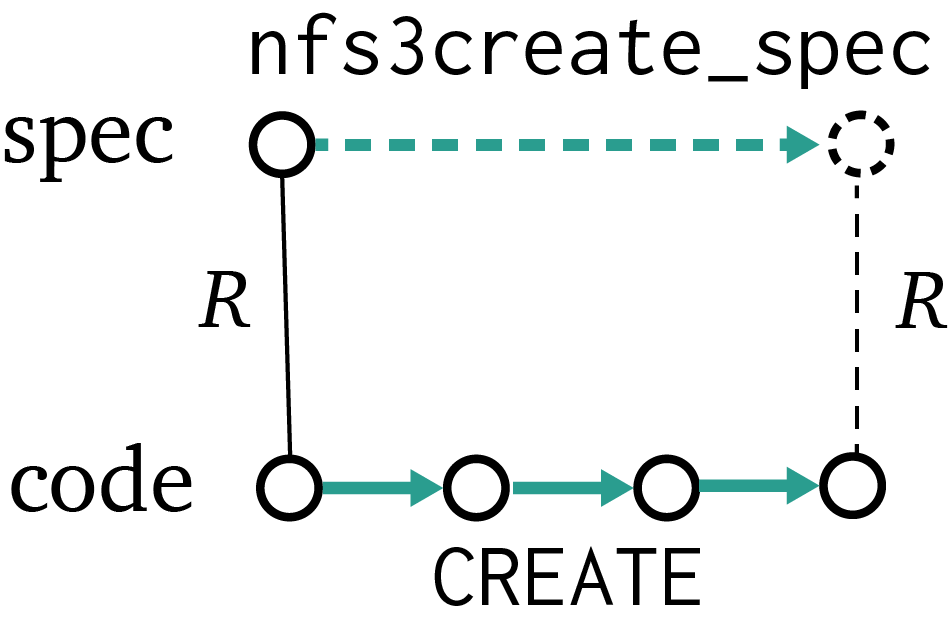
\includegraphics{fig/sequential-refinement.png}
  \end{subfigure}~~~~~\vrule~~~~%
\begin{subfigure}{0.3\textwidth}
  {\small
\begin{verbatim}

method CREATE(d_ino: uint64,
              name: Bytes)
 returns (r: Result<Ino>)
 requires R(txn_disk, fs)
 ensures R(txn_disk, fs)
 ensures r.Ok? ==>
 nfs3create_spec(d_ino, name,
   old(fs), fs, r.v)
\end{verbatim}
}
  %\caption{Dafny encoding}%
  %\label{fig:refinement:dafny}
\end{subfigure}
\vspace{0.5\baselineskip}
  \caption[Illustration of sequential refinement and its Dafny encoding]%
  {Illustration of $\seqrefinement(\infs)$ (left) and its encoding
in Dafny $\seqrefinementdfy(\infs)$ (right), for one particular operation.
In the diagram, the solid parts are assumed, and the
dashed parts must be shown to exist. The complete Dafny spec is more precise about
errors.}
  \label{fig:refinement}
\end{figure}

\begin{theorem}
  DaisyNFS atomically implements the NFS protocol, formally stated as the
  refinement $\linkedcode \refines \snfs$. Note that
  $\sdfy = \mathrm{link}(\snfs, \infs)$. Initialization falls outside the
  server's code; the caller is expected to run the \cc{Init} constructor once on
  an empty disk to establish the right $\mathrm{init}$ predicate.
  \label{thm:daisy-correctness}
\end{theorem}

\tej{make this an actual theorem re-statement (with the same number), and give
  the proof sketch here}
This theorem re-states the specification developed in
\cref{sec:daisy:refinement-spec}. Its proof is a simple on-paper argument that
connects \cref{thm:gotxn-transfer} (which \emph{assumes} a sequential
refinement) to \cref{thm:dafny} (which \emph{proves} this sequential refinement).
\Cref{fig:refinement-execs} illustrates
the intuition for this theorem in terms of an example execution of $\snfs$: the transaction system proof guarantees an
atomic execution while the sequential refinement guarantees the transactions
themselves are correct.

\begin{figure}
  \centering
  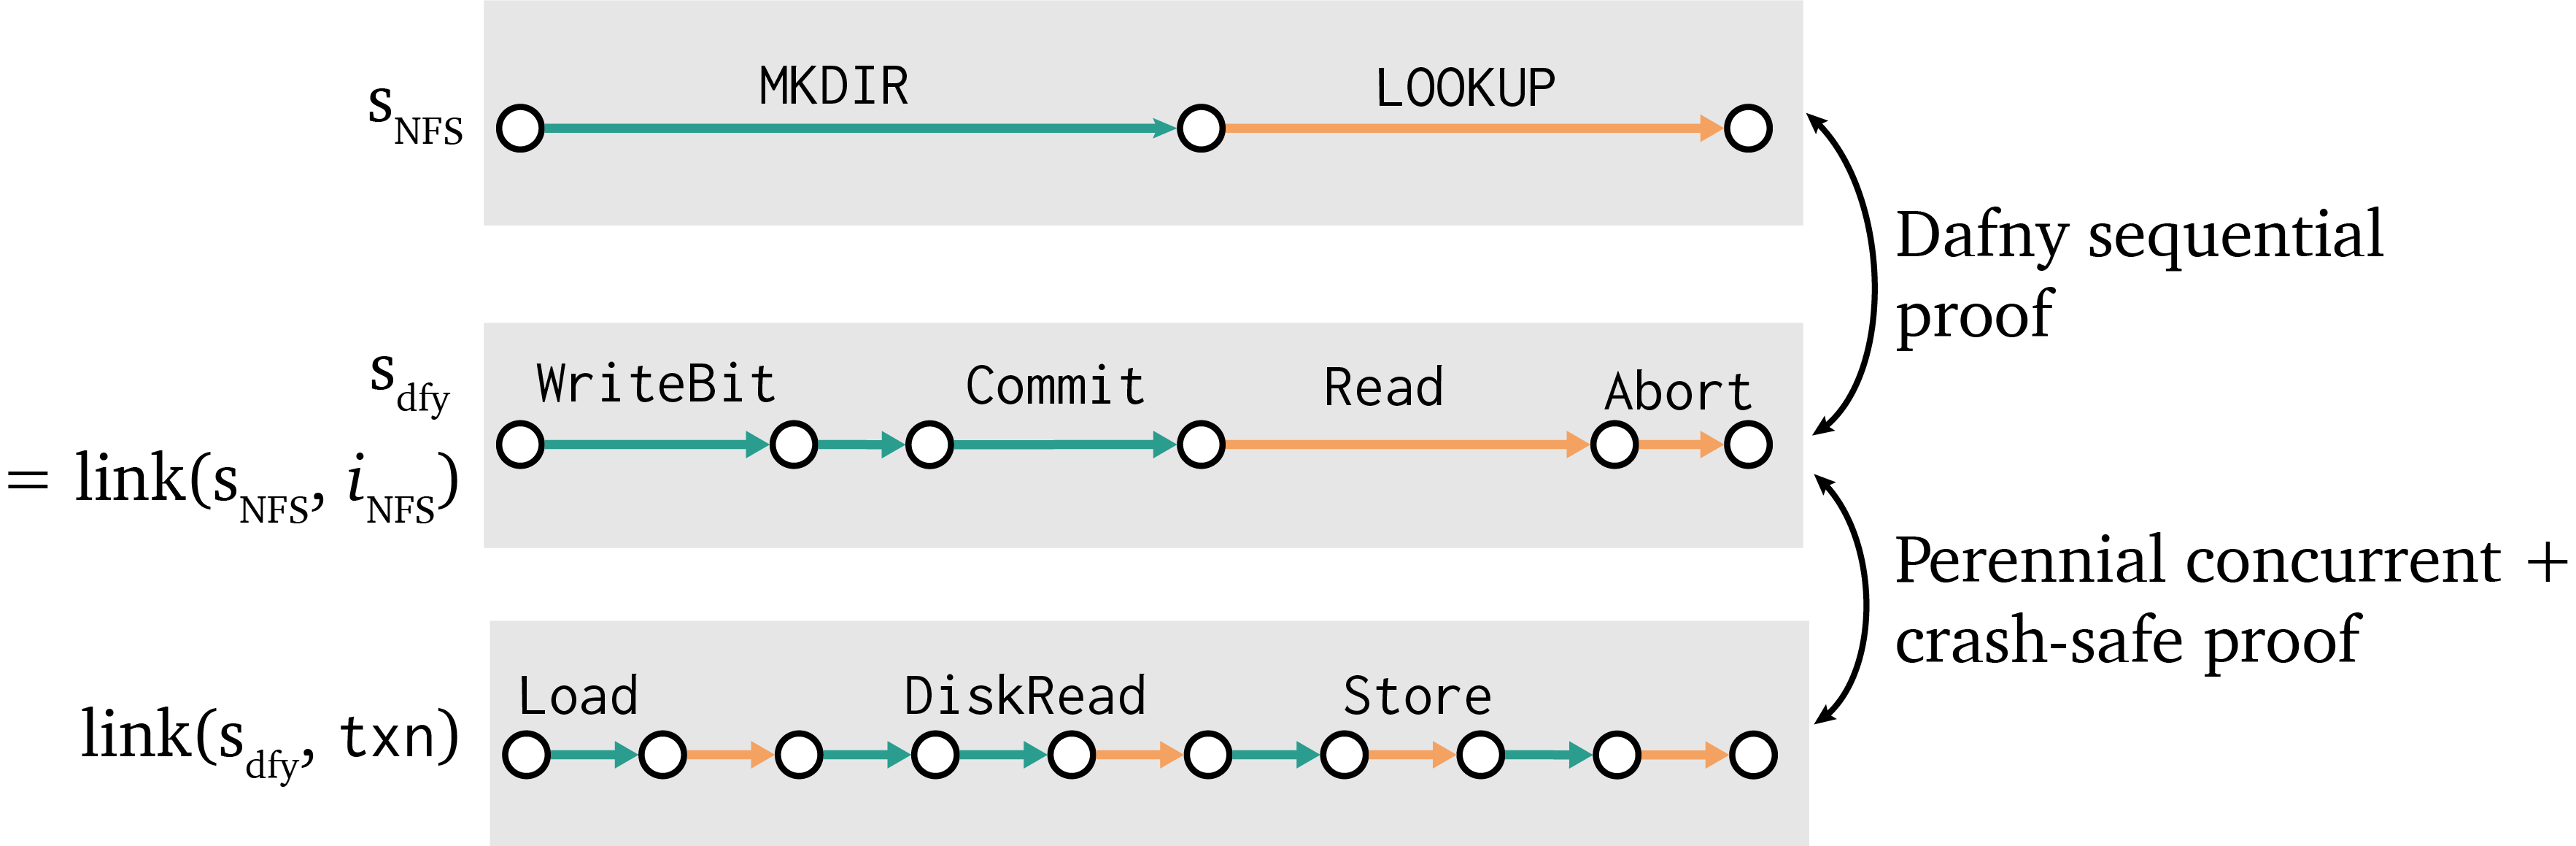
\includegraphics{fig/refinement-execs.png}
  \caption[Overall DaisyNFS proof strategy]{Illustration of the DaisyNFS proof
    strategy in terms of one
    possible execution of DaisyNFS, receiving parallel \cc{MKDIR} and \cc{LOOKUP}
    operations, at its three abstraction levels. Operations in each row are
    color-coded green or orange according to which operation they correspond to
    (the top-level \cc{MKDIR} or \cc{LOOKUP} respectively). The refinement proof first
    shows that for every code execution (bottom row), there exists an atomic
    execution at the Txn layer (middle row), as proven in
    \cref{thm:gotxn-program-refinement}. This justifies sequential reasoning to
    show the transactions on top follow the NFS specification (top row), as
    proven in \cref{thm:dafny}. Putting the two together,
    \cref{thm:daisy-correctness} shows the entire DaisyNFS server atomically
    implements the NFS specification.}
  \label{fig:refinement-execs}
\end{figure}

There are two assumptions needed for the theorems to compose. First,
$\seqrefinement_{\mathrm{dfy}}(i_{NFS})$ should imply $\seqrefinement(i_{NFS})$,
to bridge the assumption and theorem being proven in Dafny. That is, the
encoding of the refinement conditions in Dafny must be correct, but also the
semantics of the transaction system operations modeled in Dafny must match the
Coq proof. Second, every Dafny transaction must be valid, meaning
$\mathrm{safe}(i_{NFS}(op))$. Safety has a static restriction that transactions
should not modify global state, which the Dafny code satisfies because the only
mutable state in the file-system Dafny class is the transaction system, so
file-system operations cannot make mutations other than through GoTxn. The
dynamic restrictions for safety are expressed with preconditions on the GoTxn
interface so that Dafny automatically enforces them.

% We have some
% confidence this holds due to a simple check over the Dafny code: the only
% mutable state in the Dafny class that implements the file system is the ghost
% variables and the transaction system, so it cannot make mutations other than
% through GoTxn (ghost variables cannot influence execution due to the design of
% Dafny).
